\chapter{Instalación de tecnologías}
\label{anx:instalacion}


\section{AppScale}
\label{anx:inst-appscale}


\subsection{Instalación}

Antes de instalar AppScale es muy recomendable actualizar el sistema operativo. Para ello añadimos las siguientes líneas al archivo \texttt{/etc/apt/sources.list}:

\begin{lstlisting}
deb http://archive.ubuntu.com/ubuntu  lucid main restricted universe multiverse
deb http://archive.ubuntu.com/ubuntu  lucid-updates main restricted universe
deb http://security.ubuntu.com/ubuntu lucid-security main restricted universe
\end{lstlisting}

Y actualizamos el sistema operativo:

\begin{bashcode}
_: apt-get update
_: apt-get -y upgrade
\end{bashcode}

Para gestionar una infraestructura AppScale es necesario instalar una serie de programas agrupados bajo el nombre de appscale-tools. Para ello, se debe descargar el archivo \emph{tarball} de \url{http://code.google.com/p/appscale/downloads/list}. Una vez descargado, se instala:

\begin{bashcode}
_: tar xzvf appscale-tools.tar.gz
_: cd appscale-tools
_: sudo bash debian/appscale_build.sh
...
AppScale tools installation completed successfully!
\end{bashcode}

Sin olvidarse de añadir el directorio de las appscale-tools a nuestro \emph{path}:

\begin{bashcode}
_: export PATH=${PATH}:/usr/local/appscale-tools/bin
\end{bashcode}
%% Put a $ to get back highlightning in gedit

Una vez instaladas las appscale-tools instalaremos AppScale. Como lo que vamos a hacer va a ser clonar un repositorio, tenemos que asegurarnos de tener las herramientas necesarias, en este caso \texttt{git}:

\begin{bashcode}
_: apt-get -y install git-core
\end{bashcode}

y cuando esté instalado clonamos el repositorio:

\begin{bashcode}
_: cd /root/
_: git clone git://github.com/AppScale/appscale.git
\end{bashcode}

Accedemos a la carpeta recién creada y ejecutamos el \emph{script} de instalación. La instalación tarda aproximadamente una hora:

\begin{bashcode}
_: cd appscale
_: bash debian/appscale_build.sh
...
AppScale installation completed successfully!
\end{bashcode}

Nota: Si no quieres instalar todo AppScale puedes comentar las partes que no quieras en el \emph{script} de \texttt{appscale\_install.sh}. Por ejemplo, si no quieres que se instale la base de datos Voldemort, puedes comentar las líneas que hacen referencia a ella:

\begin{lstlisting}
...
all)
# scratch install of appscale including post script.
installappscaleprofile
. /etc/profile.d/appscale.sh
installgems
postinstallgems
installsetuptools
installhaproxy
postinstallhaproxy
...
installcassandra
postinstallcassandra
###installvoldemort        # No queremos Voldemort
###postinstallvoldemort    # No queremos Voldemort
installhbase
postinstallhbase
...
\end{lstlisting}


%%%%%%%%%%%%%%%%%%%%%%%%%%%%%%%%%%%%%%%%%%%%%%%%%%%%%%%%%%%%%%%%%%%%%%%%%%%%%%%%
\subsection{Comprobación de la instalación}

Para comprobar que AppScale se ha instalado correctamente lanzaremos una instancia. En primer lugar creamos un archivo llamado \texttt{ips.yaml} con el siguiente contenido (sustituye la dirección IP por la de tu máquina):

\begin{lstlisting}
--- 
:controller: 155.210.155.73
\end{lstlisting}

A continuación lanza la instancia:

\begin{bashcode}
_: appscale-run-instances --ips ips.yaml
\end{bashcode}

Si en tu navegador web vas a la dirección \texttt{http://155.210.155.73} (o la que corresponda en tu caso); allí deberías ver la página de inicio de sesión de AppScale.


\pagebreak
%%%%%%%%%%%%%%%%%%%%%%%%%%%%%%%%%%%%%%%%%%%%%%%%%%%%%%%%%%%%%%%%%%%%%%%%%%%%%%%%
\subsection{Versiones instaladas}

\begin{table}[!htbp]
\centering
   \begin{tabular}{|c|c|}
      \hline
      \textbf{Software} & \textbf{Versión} \\ \hline
      Ubuntu & 10.04 \\ \hline
      AppScale & 1.5.1 \\ \hline
      appscale-tools & 1.5 \\ \hline
   \end{tabular}
\caption{Versiones instaladas de AppScale.}
\label{table:puppet-versions}
\end{table}


\section{TORQUE}
\label{anx:inst-torque}


%%%%%%%%%%%%%%%%%%%%%%%%%%%%%%%%%%%%%%%%%%%%%%%%%%%%%%%%%%%%%%%%%%%%%%%%%%%%%%%%
\subsection{Instalación de TORQUE}


%%%%%%%%%%%%%%%%%%%%%%%%%%%%%%%%%%%%%%%%%%%%%%%%%%%%%%%%%%%%%%%%%%%%%%%%%%%%%%%%
\subsubsection{Nodo maestro}

Primero instalaremos \texttt{libssl-dev}:

\begin{bashcode}
_: apt-get install libssl-dev
\end{bashcode}

Una vez hecho esto debemos seguir las instrucciones del enlace \url{http://www.adaptivecomputing.com/resources/docs/torque/4-0-1/help.htm#topics/1-installConfig/installing.htm}, que básicamente son:

\begin{bashcode}
_: tar -xzvf torque-4.0.3.tar.gz
_: cd torque-4.0.3/
_: echo '/usr/local/lib' > /etc/ld.so.conf.d/torque.conf
_: ldconfig
_: ./configure
_: make
_: make install
\end{bashcode}


%%%%%%%%%%%%%%%%%%%%%%%%%%%%%%%%%%%%%%%%%%%%%%%%%%%%%%%%%%%%%%%%%%%%%%%%%%%%%%%%
\subsubsection{Nodos de computación}

Para crear los paquetes necesarios para los nodos de computación, haz lo siguiente:

\begin{bashcode}
_: cd torque-4.0.3/
_: make packages
\end{bashcode}

Ahora se pueden instalar estos paquetes en los nodos de computación usando los \emph{scripts} creados dentro del directorio \texttt{torque-4.0.3}:

\begin{bashcode}
_: ./torque-package-mom-linux-x86_64.sh --install
\end{bashcode}

No hay que olvidarse de incluir \texttt{/usr/local/lib} en la lista de directorios para buscar las librerías enlazadas dinámicamente:

\begin{bashcode}
_: echo '/usr/local/lib' > /etc/ld.so.conf.d/torque.conf
_: ldconfig
\end{bashcode}

Para habilitar TORQUE como un servicio se debe hacer lo siguiente:

\begin{bashcode}
_: cd torque-4.0.3
_: cp contrib/init.d/debian.pbs_mom /etc/init.d/pbs_mom
_: update-rc.d pbs_mom defaults
\end{bashcode}


%%%%%%%%%%%%%%%%%%%%%%%%%%%%%%%%%%%%%%%%%%%%%%%%%%%%%%%%%%%%%%%%%%%%%%%%%%%%%%%%
\subsection{Configuración de TORQUE}


%%%%%%%%%%%%%%%%%%%%%%%%%%%%%%%%%%%%%%%%%%%%%%%%%%%%%%%%%%%%%%%%%%%%%%%%%%%%%%%%
\subsubsection{Nodo maestro}
\label{anx:inst-torque-conf-maestro}

Añade los nodos de computación en el fichero \texttt{/var/spool/torque/server\_priv/nodes}. Por ejemplo:

\begin{lstlisting}
## This is the TORQUE server "nodes" file. 
## 
## To add a node, enter its hostname, optional processor count (np=), 
## and optional feature names.
## 
## Example:
##    host01 np=8 featureA featureB 
##    host02 np=8 featureA featureB
## 
## for more information, please visit:
## 
## http://www.clusterresources.com/torquedocs/nodeconfig.shtml

### Nodes
lucid-tor2
\end{lstlisting}

Posteriormente copia el fichero \texttt{debian.trqauthd} al directorio \texttt{/etc/init.d}:

\begin{bashcode}
_: cd torque-4.0.3/contrib/init.d
_: cp debian.trqauthd /etc/init.d
_: cd /etc/init.d
_: mv debian.trqauthd trqauthd
\end{bashcode}

Puedes empezar el demonio con:

\begin{bashcode}
_: /etc/init.d/trqauthd start
_: /usr/bin/service trqauthd start
\end{bashcode}

y puedes pararlo con:

\begin{bashcode}
_: /etc/init.d/trqauthd stop
_: /usr/bin/service trqauthd stop
\end{bashcode}

Inicializa \texttt{serverdb}:

\begin{bashcode}
_: cd torque-4.0.3/
_: ./torque.setup <user>   # Asegurate de que el usuario <user> existe en cada
                           # nodo, maestro o de computacion.
\end{bashcode}


%%%%%%%%%%%%%%%%%%%%%%%%%%%%%%%%%%%%%%%%%%%%%%%%%%%%%%%%%%%%%%%%%%%%%%%%%%%%%%%%
\subsubsection{Comprobación de la configuración}


Reiniciamos \texttt{pbs\_server} en el nodo maestro:

\begin{bashcode}
_: qterm -t quick
_: pbs_server
\end{bashcode}

Y \texttt{pbs\_mom} en los nodos de computación:

\begin{bashcode}
_: pbs_mom
\end{bashcode}

Después de esperar durante un tiempo prudencial, el comando \texttt{pbsnodes -a} proporcionará una lista de nodos libres:

\begin{bashcode}
_: pbsnodes -a
lucid-tor2
     state = free
     np = 1
     ntype = cluster
     status = rectime=1338548162,varattr=,jobs=,state=free,netload=2359153,
              gres=,loadave=0.03,ncpus=2,physmem=1023292kb,availmem=1457904kb,
              totmem=1521972kb,idletime=3003,nusers=0,nsessions=0,
              uname=Linux lucid-tor2 2.6.32-33-server
              #70-Ubuntu SMP Thu Jul 7 22:28:30 UTC 2011 x86_64,opsys=linux
     mom_service_port = 15002
     mom_manager_port = 15003
     gpus = 0
\end{bashcode}

Nota: Si el nodo aparece como \texttt{offline}, y únicamente \texttt{offline} (i.e. no como \texttt{down, offline}) se puede liberar con:

\begin{bashcode}
_: pbsnodes -c lucid-tor2
\end{bashcode}

Para ver el estado de las colas podemos ejecutar \texttt{qstat -q}:

\begin{bashcode}
_: qstat -q

server: lucid-tor1

Queue            Memory CPU Time Walltime Node  Run Que Lm  State
---------------- ------ -------- -------- ----  --- --- --  -----
batch              --      --       --      --    0   0 --   E R
                                               ----- -----
                                                   0     0
\end{bashcode}


%%%%%%%%%%%%%%%%%%%%%%%%%%%%%%%%%%%%%%%%%%%%%%%%%%%%%%%%%%%%%%%%%%%%%%%%%%%%%%%%
\subsubsection{Envío de un trabajo}

Para comprobar que TORQUE es capaz de ejecutar trabajos podemos enviarle un trabajo sencillo. Para ello ejecutaremos el comando \texttt{echo "sleep 30" | qsub} desde el usuario creado al final de la sección \ref{anx:inst-torque-conf-maestro}. Si el trabajo fue correctamente recibido deberá aparecer al usar el comando \texttt{qstat}:

\begin{bashcode}
root@lucid-tor1:~# su - david
david@lucid-tor1:~$ echo "sleep 30" | qsub
0.lucid-tor1
david@lucid-tor1:~$ qstat
Job id                    Name             User            Time Use S Queue
------------------------- ---------------- --------------- -------- - -----
0.lucid-tor1              STDIN            david                  0 Q batch
\end{bashcode}


%%%%%%%%%%%%%%%%%%%%%%%%%%%%%%%%%%%%%%%%%%%%%%%%%%%%%%%%%%%%%%%%%%%%%%%%%%%%%%%%
\subsection{Versiones instaladas}

\begin{table}[!htbp]
\centering
   \begin{tabular}{|c|c|}
      \hline
      \textbf{Software} & \textbf{Versión} \\ \hline
      Ubuntu & 10.04 \\ \hline
      TORQUE & 4.0.3 \\ \hline
   \end{tabular}
\caption{Versión instalada de TORQUE.}
\label{table:torque-versions}
\end{table}


\section{Arquitectura Web}
\label{anx:inst-web}


%%%%%%%%%%%%%%%%%%%%%%%%%%%%%%%%%%%%%%%%%%%%%%%%%%%%%%%%%%%%%%%%%%%%%%%%%%%%%%%%
\subsection{Balanceador de carga}


Usaremos nginx como balanceador de carga, y no como servidor web, que es la manera más habitual de verlo en funcionamiento.


%%%%%%%%%%%%%%%%%%%%%%%%%%%%%%%%%%%%%%%%%%%%%%%%%%%%%%%%%%%%%%%%%%%%%%%%%%%%%%%%
\subsubsection{Instalación}

Para instalar nginx, haz lo siguiente:

\begin{bashcode}
_: apt-get update
_: apt-get upgrade
_: apt-get install nginx
\end{bashcode}
\\


%%%%%%%%%%%%%%%%%%%%%%%%%%%%%%%%%%%%%%%%%%%%%%%%%%%%%%%%%%%%%%%%%%%%%%%%%%%%%%%%
\subsubsection{Configuración}

Para configurar nginx debemos añadir la parte de balanceo de carga al fichero de configuración \texttt{/etc/nginx/nginx.conf}. Como este fichero no es excesivamente grande, se muestra en su totalidad con la parte modificada resaltada:

\begin{bashcode}
user www-data;
worker_processes  1;

error_log  /var/log/nginx/error.log;
pid        /var/run/nginx.pid;

events {
    worker_connections  1024;
    # multi_accept on;
}

http {
    include       /etc/nginx/mime.types;

    access_log	/var/log/nginx/access.log;

    sendfile        on;
    #tcp_nopush     on;

    #keepalive_timeout  0;
    keepalive_timeout  65;
    tcp_nodelay        on;

    gzip  on;
    gzip_disable "MSIE [1-6]\.(?!.*SV1)";

    include /etc/nginx/conf.d/*.conf;
    include /etc/nginx/sites-enabled/*;


    ### Modified
    upstream web_servers {
      server 155.210.155.73:4567;
      server 155.210.155.178:4567;
    }

    server {
      listen 155.210.155.175:80;
      location / {
        proxy_pass http://web_servers;
      }
    }
    ### End of modification


}
\end{bashcode}
\\


%%%%%%%%%%%%%%%%%%%%%%%%%%%%%%%%%%%%%%%%%%%%%%%%%%%%%%%%%%%%%%%%%%%%%%%%%%%%%%%%
\subsubsection{Ejecución}

Para iniciar nginx haremos uso del \emph{script} localizado en \texttt{/etc/init.d}. Dicho \emph{script} puede ser usado tanto para iniciarlo:

\begin{bashcode}
_: /etc/init.d/nginx start
\end{bashcode}
\\

como para pararlo:

\begin{bashcode}
_: /etc/init.d/nginx stop
\end{bashcode}
\\


%%%%%%%%%%%%%%%%%%%%%%%%%%%%%%%%%%%%%%%%%%%%%%%%%%%%%%%%%%%%%%%%%%%%%%%%%%%%%%%%
\subsubsection{Versiones instaladas}

\begin{table}[!htbp]
\centering
   \begin{tabular}{|c|c|}
      \hline
      \textbf{Software} & \textbf{Versión} \\ \hline
      nginx & 0.7.65 \\ \hline
   \end{tabular}
\caption{Versión instalada de nginx.}
\label{table:web-mysql-versions}
\end{table}


%%%%%%%%%%%%%%%%%%%%%%%%%%%%%%%%%%%%%%%%%%%%%%%%%%%%%%%%%%%%%%%%%%%%%%%%%%%%%%%%


\subsection{Servidor web}


Como servidor web usaremos WEBrick, que es el servidor web que viene por defecto con la instalación de Ruby. Instalando Ruby instalaremos a la vez el servidor web.


%%%%%%%%%%%%%%%%%%%%%%%%%%%%%%%%%%%%%%%%%%%%%%%%%%%%%%%%%%%%%%%%%%%%%%%%%%%%%%%%
\subsubsection{Instalación}

Lo primero que hay que hacer es instalar Ruby y RubyGems. Para ello, consulta el anexo \ref{anx:inst-ruby} de instalación de Ruby.

Una vez instalado Ruby y RubyGems, instalaremos el paquete \texttt{ruby-dev}:

\begin{bashcode}
_: apt-get install ruby1.8-dev
\end{bashcode}
\\

Y ahora instalaremos el soporte necesario para interactuar con la base de datos:

\begin{bashcode}
_: apt-get install libmysqlclient-dev
_: gem install mysql
\end{bashcode}
\\

La aplicación web será desarrollada usando Sinatra. Antes de comenzar con la instalación, comprueba que tu versión de RubyGems es igual o superior a la 1.3.6. Esto puede hacerse fácilmente de la siguiente manera:

\begin{bashcode}
_: gem --version
1.3.6
\end{bashcode}
\\

Para instalar Sinatra, haremos lo siguiente:

\begin{bashcode}
_: gem install sinatra
Successfully installed rack-1.4.1
Successfully installed rack-protection-1.2.0
Successfully installed tilt-1.3.3
Successfully installed sinatra-1.3.2
4 gems installed
Installing ri documentation for rack-1.4.1...
...
Installing ri documentation for sinatra-1.3.2...
Installing RDoc documentation for rack-1.4.1...
...
Installing RDoc documentation for sinatra-1.3.2...
\end{bashcode}
\\

Nota: Puede llevar un tiempo hasta que el proceso de instalación muestre cosas por pantalla.


%%%%%%%%%%%%%%%%%%%%%%%%%%%%%%%%%%%%%%%%%%%%%%%%%%%%%%%%%%%%%%%%%%%%%%%%%%%%%%%%
\subsubsection{Ejecución}

Una vez que la instalación ha finalizado, vamos a crear la primera aplicación web. Guarda el siguiente fichero como \texttt{web.rb}:

\begin{rubycode}
require 'rubygems'
require 'sinatra'

get '/' do
  'Hello world!'
end
\end{rubycode}

y lanza el servidor web:

\begin{bashcode}
_: ruby web.rb
\end{bashcode}
\\

Nota: Para salir Ctrl + C.

En tu navegador web preferido ve a la dirección \texttt{http://localhost:4567} y encontrarás la aplicación web que acabamos de crear.


%%%%%%%%%%%%%%%%%%%%%%%%%%%%%%%%%%%%%%%%%%%%%%%%%%%%%%%%%%%%%%%%%%%%%%%%%%%%%%%%
\subsubsection{Añadiendo soporte para la base de datos}

Para interactuar con la base de datos usaremos ActiveRecord. Este componente es parte de Ruby On Rails, pero también existe como una \emph{gem} independiente. Vamos a instalarla:

\begin{bashcode}
_: gem install activerecord
\end{bashcode}
\\

Ahora vamos a crear una segunda aplicación web. Guarda el siguiente fichero como \texttt{web2.rb}:

\begin{rubycode}
require 'rubygems'
require 'sinatra'
require 'active_record'

class Article < ActiveRecord::Base
end

get '/' do
   'Hello there!'
end
\end{rubycode}

y lanza el servidor web como antes:

\begin{bashcode}
_: ruby web2.rb
\end{bashcode}
\\

En tu navegador web ve a la dirección \texttt{http://localhost:4567} y encontrarás la aplicación web. Muestra lo mismo que la primera aplicación web, pero hemos incluido (aunque no usado) el soporte para la base de datos.


%%%%%%%%%%%%%%%%%%%%%%%%%%%%%%%%%%%%%%%%%%%%%%%%%%%%%%%%%%%%%%%%%%%%%%%%%%%%%%%%
\subsubsection{Versiones instaladas}

\begin{table}[!htbp]
\centering
   \begin{tabular}{|c|c|}
      \hline
      \textbf{Software} & \textbf{Versión} \\ \hline
      Ruby & 1.8.7 \\ \hline
      RubyGems & 1.8.21 \\ \hline
      Sinatra & 1.3.2 \\ \hline
      ActiveRecord & 3.2.3 \\ \hline
   \end{tabular}
\caption{Versiones instaladas de Ruby, RubyGems, Sinatra y ActiveRecord.}
\label{table:web-mysql-versions}
\end{table}


%%%%%%%%%%%%%%%%%%%%%%%%%%%%%%%%%%%%%%%%%%%%%%%%%%%%%%%%%%%%%%%%%%%%%%%%%%%%%%%%


\subsection{Base de datos}


Como servidor de base de datos usaremos MySQL.


%%%%%%%%%%%%%%%%%%%%%%%%%%%%%%%%%%%%%%%%%%%%%%%%%%%%%%%%%%%%%%%%%%%%%%%%%%%%%%%%
\subsubsection{Instalación}

Para instalar MySQL, haz lo siguiente:

\begin{bashcode}
_: apt-get install mysql-server
\end{bashcode}
\\


%%%%%%%%%%%%%%%%%%%%%%%%%%%%%%%%%%%%%%%%%%%%%%%%%%%%%%%%%%%%%%%%%%%%%%%%%%%%%%%%
\subsubsection{Configuración}

Para configurar los ajustes básicos hay que editar el fichero \texttt{/etc/mysql/my.cnf}. Por ejemplo, si vamos a aceptar conexiones de otra máquina, hay que modificar el parámetro \texttt{bind\_address}. En nuestro caso, lo modificaremos para aceptar conexiones del servidor web:

\begin{bashcode}
bind_address = 155.210.155.73
\end{bashcode}
\\

Nota: Si estás usando Ubuntu 10.04 debido a un \emph{bug} \href{http://ubuntuforums.org/showthread.php?t=1479310}{es mejor que comentes toda la línea}. Además nosotros usaremos dos servidores web, así que mejor la comentamos:

\begin{bashcode}
#bind_address = 155.210.155.73
\end{bashcode}
\\

Vamos a reiniciar el servidor para que los cambios surtan efecto:

\begin{bashcode}
_: /usr/bin/service mysql restart
\end{bashcode}
\\

Para comprobar que ha sido instalado correctamente, podemos hacer lo siguiente:

\begin{bashcode}
_: mysql -u root -p     # Introduce MySQL's root password
Welcome to the MySQL monitor.  Commands end with ; or \g.
Your MySQL connection id is 34
Server version: 5.1.61-0ubuntu0.10.04.1 (Ubuntu)
...
Type 'help;' or '\h' for help. Type '\c' to clear the current input statement.

mysql> CREATE DATABASE mydb;
\end{bashcode}
\\


%%%%%%%%%%%%%%%%%%%%%%%%%%%%%%%%%%%%%%%%%%%%%%%%%%%%%%%%%%%%%%%%%%%%%%%%%%%%%%%%
\subsubsection{Ejecución}

Para ejecutar el servidor de bases de datos usaremos el programa \texttt{service} localizado en \texttt{/usr/bin/service}. Sirve tanto para iniciarlo:

\begin{bashcode}
_: /usr/bin/service mysql start
\end{bashcode}
\\

como para pararlo:
\begin{bashcode}
_: /usr/bin/service mysql stop
\end{bashcode}
\\


%%%%%%%%%%%%%%%%%%%%%%%%%%%%%%%%%%%%%%%%%%%%%%%%%%%%%%%%%%%%%%%%%%%%%%%%%%%%%%%%
\subsubsection{Versiones instaladas}

\begin{table}[!htbp]
\centering
   \begin{tabular}{|c|c|}
      \hline
      \textbf{Software} & \textbf{Versión} \\ \hline
      mysql & 5.1.61 \\ \hline
   \end{tabular}
\caption{Versión instalada de MySQL.}
\label{table:web-mysql-versions}
\end{table}


\section{Ruby}
\label{anx:inst-ruby}

Antes de poder programar en el lenguaje de programación Ruby deberemos instalar una serie de paquetes. Además de la instalación de los elementos necesarios para programar en Ruby también se instalarán una serie de herramientas de ayuda.


%%%%%%%%%%%%%%%%%%%%%%%%%%%%%%%%%%%%%%%%%%%%%%%%%%%%%%%%%%%%%%%%%%%%%%%%%%%%%%%%
\subsection{Instalación}

Empezaremos instalando Ruby, IRB (Interactive Ruby Shell) y RDoc, la herramienta de generación de documentación de Ruby:

\begin{bashcode}
_: apt-get install ruby irb rdoc
\end{bashcode}

A continuación instalaremos RubyGems. Para ello, descarga el paquete más actual de \href{http://rubyforge.org/frs/?group_id=126}{rubyforge}. Durante el resto de la instalación usaremos como ejemplo el paquete 1.8.10, pero los pasos son análogos para cualquier otra versión.

Descomprimimos el paquete:

\begin{bashcode}
_: tar xvf rubygems-1.8.10.tgz
\end{bashcode}

E instalamos RubyGems:

\begin{bashcode}
_: cd rubygems-1.8.10
_: ruby setup.rb
\end{bashcode}

Una vez instalado, comprobamos la versión:

\begin{bashcode}
_: gem --version
1.8.10
\end{bashcode}

Y la actualizamos a la última versión disponible. Es posible que antes de hacer este paso haya que actualizar el sistema operativo.

\begin{bashcode}
_: gem update --system
_: gem --version
1.8.24
\end{bashcode}

En caso de que sea necesario actualizar el sistema operativo, se hace de esta manera:

\begin{bashcode}
_: apt-get upgrade
\end{bashcode}


%%%%%%%%%%%%%%%%%%%%%%%%%%%%%%%%%%%%%%%%%%%%%%%%%%%%%%%%%%%%%%%%%%%%%%%%%%%%%%%%
\subsection{Problemas}

Puede que durante la ejecución de programas Ruby, o la instalación de \emph{gems} te encuentres con el siguiente error: \texttt{`require': no such file to load -- mkmf (LoadError)}. La manera de solucionarlo es instalando el paquete \texttt{ruby1.8-dev}:

\begin{bashcode}
_: apt-get install ruby1.8-dev
\end{bashcode}

También puede aparecer el error \texttt{no such file to load -- net/https (LoadError)}. Para solucionarlo, instala \texttt{libopenssl-ruby}:

\begin{bashcode}
_: apt-get install libopenssl-ruby
\end{bashcode}


\pagebreak
%%%%%%%%%%%%%%%%%%%%%%%%%%%%%%%%%%%%%%%%%%%%%%%%%%%%%%%%%%%%%%%%%%%%%%%%%%%%%%%%
\subsection{Versiones instaladas}

\begin{table}[!htbp]
\centering
   \begin{tabular}{|c|c|}
      \hline
      \textbf{Software} & \textbf{Versión} \\ \hline
      Ubuntu & 10.04 \\ \hline
      Ruby & 1.8.7 \\ \hline
      RubyGems & 1.8.10 (o superior) \\ \hline
   \end{tabular}
\caption{Versiones instaladas de Ruby y RubyGems.}
\label{table:ruby-versions}
\end{table}


\section{Libvirt}
\label{anx:inst-libvirt}

%%%%%%%%%%%%%%%%%%%%%%%%%%%%%%%%%%%%%%%%%%%%%%%%%%%%%%%%%%%%%%%%%%%%%%%%%%%%%%%%
\subsection{Instalación}

Instalaremos \texttt{libvirt-ruby} mediante apt-get:

\begin{bashcode}
_: apt-get install libvirt-ruby
\end{bashcode}


%%%%%%%%%%%%%%%%%%%%%%%%%%%%%%%%%%%%%%%%%%%%%%%%%%%%%%%%%%%%%%%%%%%%%%%%%%%%%%%%
\subsection{Versiones instaladas}

\begin{table}[!htbp]
\centering
   \begin{tabular}{|c|c|}
      \hline
      \textbf{Software} & \textbf{Versión} \\ \hline
      Ubuntu & 10.04 \\ \hline
      Ruby & 1.8.7 \\ \hline
      libvirt-ruby & 0.0.7-1 \\ \hline
   \end{tabular}
\caption{Versión instalada de libvirt.}
\label{table:libvirt-versions}
\end{table}


\section{MCollective}
\label{anx:inst-mcollective}


MCollective es un sistema de despliegue de servidores y de sistemas de ejecución de trabajos en paralelo. Su función principal dentro del ámbito de la administración de sistemas es la ejecución de una acción sobre un conjunto de servidores. Para lograr esto, MCollective se apoya en un \emph{middleware} que proporciona un servicio publicador-suscriptor. En este tipo de programas, las publicaciones y suscripciones suelen implementarse mediante el paso de mensajes asíncrono. Una de las posibilidades que se pueden usar con MCollective es RabbitMQ (Anexo \ref{anx:inst-rabbitmq}), que implementa el estándar de paso de mensajes AMQP (Advanced Message Queuing Protocol).

Dentro de la arquitectura MCollective, los componentes más importantes son:
\begin{itemize}
\item Cliente: Indica las órdenes a ejecutar.
\item \emph{Middleware}: Lleva las órdenes del cliente a los servidores.
\item Servidor: Cumple las órdenes que le son enviadas.
\end{itemize}

El funcionamiento habitual de MCollective consiste en el lanzamiento de una orden desde el cliente que es transmitida a todos los servidores (\emph{broadcast}) y éstos la llevan a cabo. En la figura \ref{figure:arquitectura-mcollective} se puede apreciar como la instrucción emitida por el cliente llega al corredor de mensajes (\emph{broker}) y éste lo hace llegar a los servidores para que la cumplan.

\begin{figure} [!htbp]
  \centering
  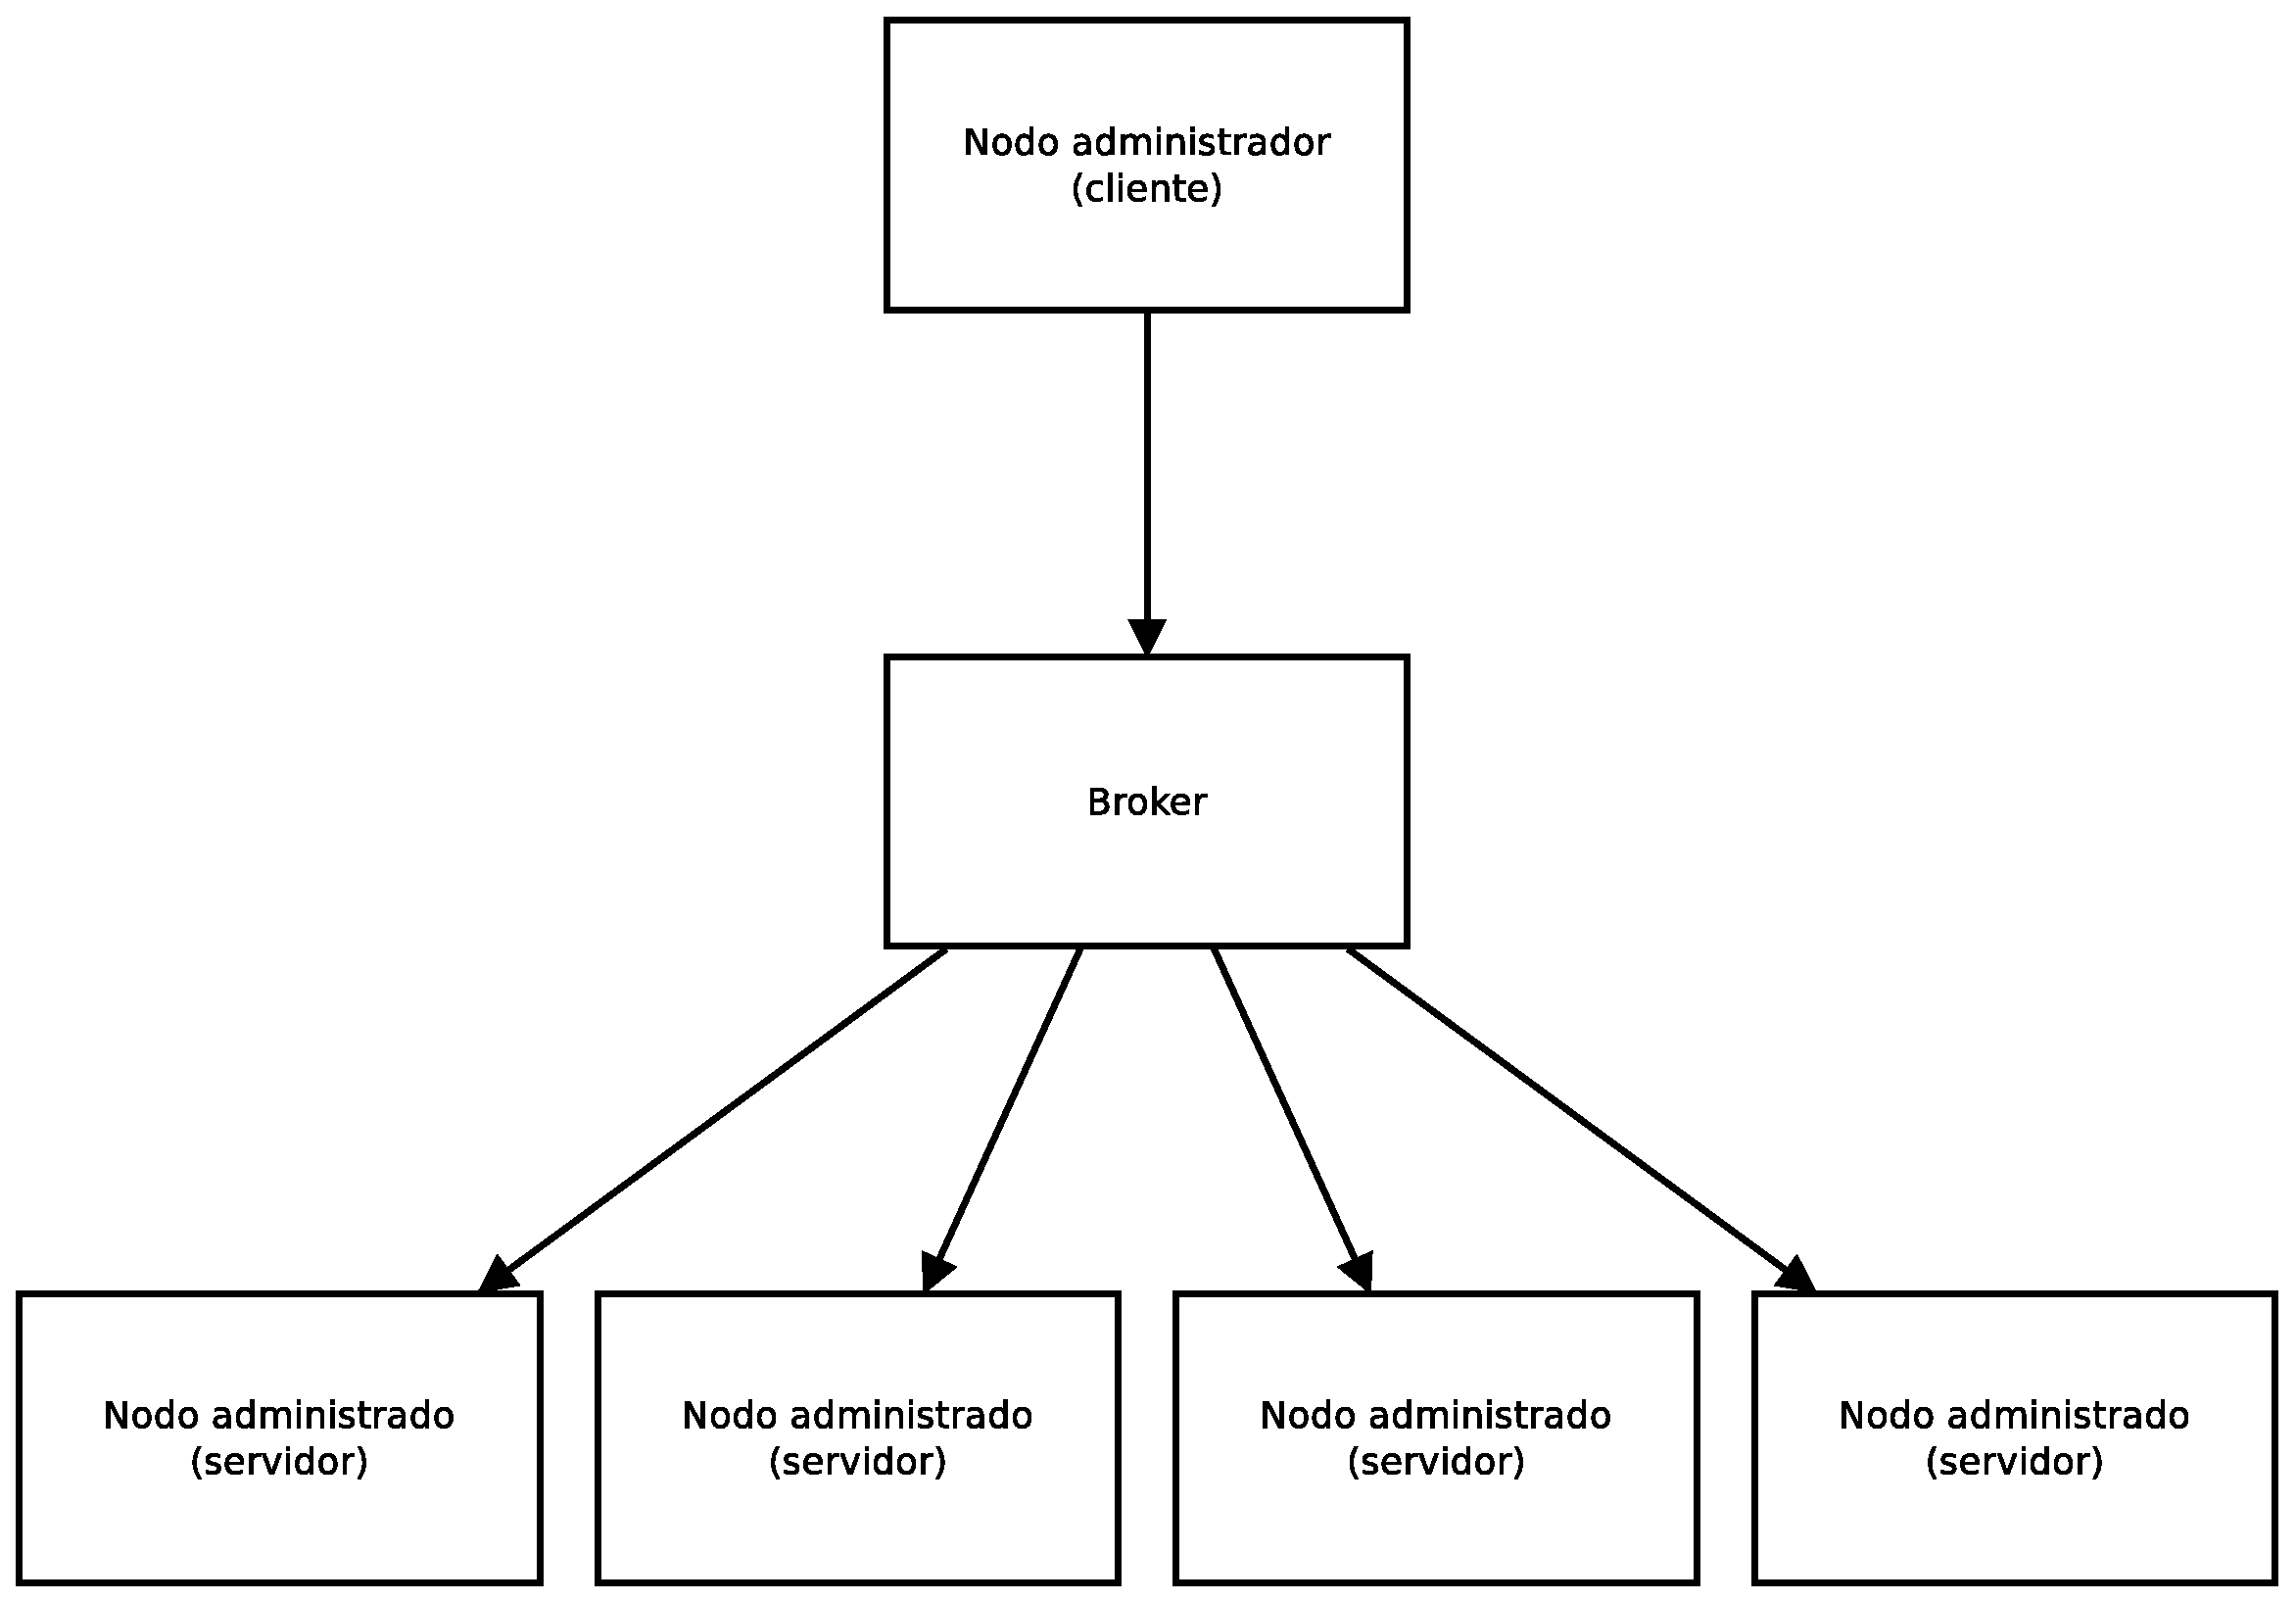
\includegraphics[width=13.5cm]{figuras/Arquitectura_MCollective.eps}
  \caption{Arquitectura de MCollective.}
\label{figure:arquitectura-mcollective}
\end{figure}

%%%%%%%%%%%%%%%%%%%%%%%%%%%%%%%%%%%%%%%%%%%%%%%%%%%%%%%%%%%%%%%%%%%%%%%%%%%%%%%%
\subsection{Instalación}

El primer paso consiste en la instalación de RubyGems. Para ello, consulta el anexo \ref{anx:inst-ruby} de instalación de Ruby y RubyGems.

Descargamos los paquetes \texttt{mcollective}, \texttt{mcollective-client} y \texttt{mcollective-common} de \url{http://downloads.puppetlabs.com/mcollective/}:

\begin{bashcode}
_: wget http://downloads.puppetlabs.com/mcollective/\
mcollective_1.2.1-1_all.deb
_: wget http://downloads.puppetlabs.com/mcollective/\
mcollective-client_1.2.1-1_all.deb
_: wget http://downloads.puppetlabs.com/mcollective/\
mcollective-common_1.2.1-1_all.deb
\end{bashcode}

Dependiendo de si el nodo va a ser administrador o administrado tendremos que instalar unos u otros paquetes:

\begin{tabular}{|c|c|c|}
   \hline
   Paquete & Nodo administrador & Nodo administrado \\ \hline
   mcollective-common & X & X \\ \hline
   mcollective-client & X &   \\ \hline
   mcollective &  & X \\ \hline
\end{tabular}
\\

Podemos instalar los paquetes de la siguiente manera:

\begin{bashcode}
_: dpkg -i mcollective*.deb
\end{bashcode}

Una vez instalado MCollective, instalamos la librería \texttt{libstomp-ruby}:

\begin{bashcode}
_: apt-get install libstomp-ruby
\end{bashcode}


%%%%%%%%%%%%%%%%%%%%%%%%%%%%%%%%%%%%%%%%%%%%%%%%%%%%%%%%%%%%%%%%%%%%%%%%%%%%%%%%
\subsection{Configuración}

A continuación hay que editar el fichero de configuración de MCollective. En los nodos administradores (clientes) se encuentra en \texttt{/etc/mcollective/client.cfg} mientras que en los nodos administrados (servidores) se encuentra en \texttt{/etc/mcollective/server.cfg}. Nos aseguramos de que contengan los siguientes valores:

\begin{bashcode}
plugin.stomp.host = 155.210.155.ABC # Direccion IP del MQ broker
plugin.stomp.port = 61613
plugin.stomp.user = mcollective
plugin.stomp.password = mcollective
\end{bashcode}


%%%%%%%%%%%%%%%%%%%%%%%%%%%%%%%%%%%%%%%%%%%%%%%%%%%%%%%%%%%%%%%%%%%%%%%%%%%%%%%%
\subsection{Comprobación de la instalación}

En el servidor stomp lanza el siguiente comando:

\begin{bashcode}
_: /usr/sbin/service rabbitmq-server start
\end{bashcode}

En los nodos administrados (servidores) lanza éste:

\begin{bashcode}
_: /usr/sbin/service mcollective start
\end{bashcode}

Y en uno de los nodos administradores (clientes) lanzaremos el comando \texttt{mc-ping}. La salida obtenida al ejecutar el comando debería ser similar a la siguiente:

\begin{bashcode}
_: mc-ping
155.210.155.177                       time=46.06 ms
---- ping statistics ----
1 replies max: 46.06 min: 46.06 avg: 46.06
\end{bashcode}


%%%%%%%%%%%%%%%%%%%%%%%%%%%%%%%%%%%%%%%%%%%%%%%%%%%%%%%%%%%%%%%%%%%%%%%%%%%%%%%%
\subsection{Versiones instaladas}

\begin{table}[!htbp]
\centering
   \begin{tabular}{|c|c|}
      \hline
      \textbf{Software} & \textbf{Versión} \\ \hline
      Ubuntu & 10.04 \\ \hline
      MCollective & 1.2.1-1 \\ \hline
      libstomp-ruby & 1.8 (1.0.4-1) \\ \hline
   \end{tabular}
\caption{Versiones instaladas de MCollective y libstomp.}
\label{table:mcollective-versions}
\end{table}


\section{RabbitMQ}
\label{anx:inst-rabbitmq}


RabbitMQ es un \emph{middleware} de mensajería que implementa el estándar AMQP (Advanced Message Queuing Protocol).


%%%%%%%%%%%%%%%%%%%%%%%%%%%%%%%%%%%%%%%%%%%%%%%%%%%%%%%%%%%%%%%%%%%%%%%%%%%%%%%%
\subsection{Instalación de RabbitMQ}

Empezaremos añadiendo la línea

\begin{bashcode}
deb http://www.rabbitmq.com/debian/ testing main
\end{bashcode}

a nuestro fichero \texttt{/etc/apt/sources.list} de la siguiente manera:

\begin{bashcode}
_: echo "deb http://www.rabbitmq.com/debian/ testing main" >> \
/etc/apt/sources.list
\end{bashcode}

Para evitar avisos acerca de paquetes que no han sido firmados, podemos añadir la clave pública de RabbitMQ a nuestra lista de claves:

\begin{bashcode}
_: wget http://www.rabbitmq.com/rabbitmq-signing-key-public.asc
_: apt-key add rabbitmq-signing-key-public.asc
\end{bashcode}

Actualizamos el sistema con los nuevos cambios:

\begin{bashcode}
_: apt-get update
\end{bashcode}

E instalamos el paquete de la manera habitual:

\begin{bashcode}
_: apt-get install rabbitmq-server
\end{bashcode}

La instalación incluirá automáticamente los paquetes de Erlang necesarios para ejecutar RabbitMQ.


%%%%%%%%%%%%%%%%%%%%%%%%%%%%%%%%%%%%%%%%%%%%%%%%%%%%%%%%%%%%%%%%%%%%%%%%%%%%%%%%
\subsection{Instalación de los \emph{plugins} para el soporte de AMQP y STOMP}

RabbitMQ no basta para proporcionar el servicio de paso de mensajes que MCollective requiere. Para que sea capaz de proporcionarlo necesitamos instalar unos \emph{plugins}. Para ello, vamos al fichero \texttt{/usr/lib/rabbitmq/lib/rabbitmq\_server-2.7.1/plugins} y comprobamos si existen \texttt{amqp\_client-2.7.1.ez} y \texttt{rabbitmq\_stomp-2.7.1.ez}. Si no existen, los instalamos:

\begin{bashcode}
_: wget -q http://www.rabbitmq.com/releases/plugins/v2.7.1/\
amqp_client-2.7.1.ez
_: wget -q http://www.rabbitmq.com/releases/plugins/v2.7.1/\
rabbitmq_stomp-2.7.1.ez
\end{bashcode}

Nota: Los nombres de los \emph{plugins} pueden variar dependiendo de la versión instalada.

Activamos los \emph{plugins}:

\begin{bashcode}
_: rabbitmq-plugins list
_: rabbitmq-plugins enable amqp_client           # El nombre puede cambiar
_: rabbitmq-plugins enable rabbitmq_stomp        # El nombre puede cambiar
\end{bashcode}

y reiniciamos el servidor:

\begin{bashcode}
_: /usr/sbin/service rabbitmq-server restart
\end{bashcode}


%%%%%%%%%%%%%%%%%%%%%%%%%%%%%%%%%%%%%%%%%%%%%%%%%%%%%%%%%%%%%%%%%%%%%%%%%%%%%%%%
\subsection{Configuración de la cuenta de MCollective}

Añadimos el usuario \texttt{mcollective} y la contraseña \texttt{mcollective}:
\begin{bashcode}
_: rabbitmqctl add_user mcollective mcollective
\end{bashcode}

Establecemos los permisos necesarios:

\begin{bashcode}
_: rabbitmqctl set_permissions -p / mcollective "^amq.gen-.*" ".*" ".*"
\end{bashcode}

Y por seguridad borramos la cuenta de invitado:

\begin{bashcode}
_: rabbitmqctl delete_user guest
\end{bashcode}


%%%%%%%%%%%%%%%%%%%%%%%%%%%%%%%%%%%%%%%%%%%%%%%%%%%%%%%%%%%%%%%%%%%%%%%%%%%%%%%%
\subsection{Comprobación de la instalación}

Para comprobar que hemos instalado correctamente RabbitMQ podemos hacer lo siguiente:

\begin{bashcode}
_: invoke-rc.d rabbitmq-server start
Starting rabbitmq-server: SUCCESS
rabbitmq-server.
\end{bashcode}


%%%%%%%%%%%%%%%%%%%%%%%%%%%%%%%%%%%%%%%%%%%%%%%%%%%%%%%%%%%%%%%%%%%%%%%%%%%%%%%%
\subsection{Versiones instaladas}

\begin{table}[!htbp]
\centering
   \begin{tabular}{|c|c|}
      \hline
      \textbf{Software} & \textbf{Versión} \\ \hline
      Ubuntu & 10.04 \\ \hline
      RabbitMQ & 2.7.1 \\ \hline
      Erlang & R13B03 (erts-5.7.4) \\ \hline
   \end{tabular}
\caption{Versiones instaladas de RabbitMQ y Erlang.}
\label{table:rabbitmq-versions}
\end{table}


\section{Puppet}
\label{anx:inst-puppet}


%%%%%%%%%%%%%%%%%%%%%%%%%%%%%%%%%%%%%%%%%%%%%%%%%%%%%%%%%%%%%%%%%%%%%%%%%%%%%%%%
\subsection{Instalación de libopenssl-ruby}

Si nuestro sistema no tiene instalado \texttt{libopenssl-ruby} tenemos que instalarlo:

\begin{bashcode}
_: apt-get install libopenssl-ruby
\end{bashcode}


%%%%%%%%%%%%%%%%%%%%%%%%%%%%%%%%%%%%%%%%%%%%%%%%%%%%%%%%%%%%%%%%%%%%%%%%%%%%%%%%
\subsection{Creación del entorno de instalación de Puppet}

Puppet necesita para su correcto funcionamiento una herramienta llamada Facter. Esta herramienta permite obtener datos como el sistema operativo, la distribución de Linux o la dirección MAC de un ordenador. Antes de instalar Facter y Puppet, hay que dar valores a ciertas variables:

\begin{bashcode}
_: FACTER_DIR="/root/facter-1.6.4"
_: PUPPET_DIR="/root/puppet-2.7.9"
_: PATH=$PATH:$FACTER_DIR/bin:$PUPPET_DIR/puppet/bin
_: RUBYLIB=$FACTER_DIR/lib:$PUPPET_DIR/lib
_: export PATH RUBYLIB
\end{bashcode}


%% Put a $ to get back highlightning in gedit
%%%%%%%%%%%%%%%%%%%%%%%%%%%%%%%%%%%%%%%%%%%%%%%%%%%%%%%%%%%%%%%%%%%%%%%%%%%%%%%%
\subsection{Instalación de Facter}

Instalaremos Facter mediante una instalación por fuentes. Para ello primero tenemos que obtener las fuentes:

\begin{bashcode}
_: wget http://puppetlabs.com/downloads/facter/facter-1.6.4.tgz
\end{bashcode}

Una vez conseguidas las fuentes lo descomprimimos:

\begin{bashcode}
_: gzip -d -c facter-1.6.4.tgz | tar xf -
\end{bashcode}

Y posteriormente lo instalamos:

\begin{bashcode}
_: cd facter-1.6.4
_: ruby install.rb
\end{bashcode}


%%%%%%%%%%%%%%%%%%%%%%%%%%%%%%%%%%%%%%%%%%%%%%%%%%%%%%%%%%%%%%%%%%%%%%%%%%%%%%%%
\subsection{Instalación de Puppet}

Instalaremos Puppet también mediante fuentes. Obtenemos las fuentes:

\begin{bashcode}
_: wget http://puppetlabs.com/downloads/puppet/puppet-2.7.9.tgz
\end{bashcode}

Lo descomprimimos:

\begin{bashcode}
_: gzip -d -c puppet-2.7.9.tgz | tar xf -
\end{bashcode}

Y lo instalamos:

\begin{bashcode}
_: cd puppet-2.7.9
_: ruby install.rb
\end{bashcode}


%%%%%%%%%%%%%%%%%%%%%%%%%%%%%%%%%%%%%%%%%%%%%%%%%%%%%%%%%%%%%%%%%%%%%%%%%%%%%%%%
\subsection{Configuración de Puppet}

Nos aseguramos de que el fichero \texttt{/etc/puppet/puppet.conf} existe en nuestro sistema. Si no es así, podemos crearlo de la siguiente manera:

\begin{bashcode}
_: puppetmasterd --genconfig > /etc/puppet/puppet.conf
\end{bashcode}

Tenemos que asegurarnos de que existen tanto un usuario como un grupo \texttt{puppet}. Si no existen, los creamos:

\begin{bashcode}
_: groupadd puppet
_: useradd -g puppet puppet
\end{bashcode}

Por último tenemos que asegurarnos de que el directorio \texttt{/var/lib/puppet/rrd} pertenece al usuario y grupo \texttt{puppet}. Si no pertenece, cambiamos los permisos:

\begin{bashcode}
_: chown puppet /var/lib/puppet/rrd
_: chgrp puppet /var/lib/puppet/rrd
\end{bashcode}

Nota: Si este directorio todavía no existe seguimos adelante con la instalación y ya revisitaremos este punto.


%%%%%%%%%%%%%%%%%%%%%%%%%%%%%%%%%%%%%%%%%%%%%%%%%%%%%%%%%%%%%%%%%%%%%%%%%%%%%%%%
\subsection{Comprobación de la instalación}

Vamos a comprobar de manera rápida que la instalación de Facter y Puppet fue exitosa:

\begin{bashcode}
_: facter
[Muestra datos del sistema]
_: puppet describe -s user
[Muestra una descripcion del tipo usuario]
\end{bashcode}

Ahora creamos un manifiesto simple en el fichero \texttt{manifest.pp}:

\begin{rubycode}
file {'testfile':
  path    => '/tmp/testfile',
  ensure  => present,
  mode    => 0640,
  content => "I'm a test file.",
}
\end{rubycode}

Lo aplicamos:

\begin{bashcode}
_: puppet apply manifest.pp
\end{bashcode}

Y comprobamos el contenido del fichero \texttt{/tmp/testfile} que Puppet debería haber creado:

\begin{bashcode}
_: cat /tmp/testfile
I'm a test file.
\end{bashcode}

Ahora es momento de volver al directorio \texttt{/var/lib/puppet/rrd} y comprobar que tanto el usuario como el grupo de ese directorio tienen como valor \texttt{puppet}.


%%%%%%%%%%%%%%%%%%%%%%%%%%%%%%%%%%%%%%%%%%%%%%%%%%%%%%%%%%%%%%%%%%%%%%%%%%%%%%%%
\subsubsection{Comprobación del maestro de Puppet}

Para comprobar que el maestro de puppet puede ejecutarse como un demonio tenemos que hacer:

\begin{bashcode}
_: puppet master
Could not prepare for execution: Got 1 failure(s) while initializing: \
change from directory to file failed: 
Could not set 'file on ensure: Is a directory - /var/lib/puppet/facts
\end{bashcode}

Si aparece este fallo tenemos que ir al fichero de configuración \texttt{/etc/puppet/puppet.conf} y comentar la línea con la propiedad \texttt{factdest}. Esta es la solución propuesta para el \href{https://projects.puppetlabs.com/issues/9491}{bug}.

Si lo ejecutamos de nuevo no debería dar más problemas:

\begin{bashcode}
_: puppet master
\end{bashcode}


%%%%%%%%%%%%%%%%%%%%%%%%%%%%%%%%%%%%%%%%%%%%%%%%%%%%%%%%%%%%%%%%%%%%%%%%%%%%%%%%
\subsubsection{Comprobación del agente de Puppet}

Nota: Supondremos que el maestro de Puppet se está ejecutando en una máquina que tiene por nombre \texttt{puppet.example.com}. La máquina desde la que se ejecuta el agente tiene por nombre \texttt{node1.example.com}

Desde la máquina que tiene el agente, lanzamos la siguiente orden:

\begin{bashcode}
_: puppet agent --server=puppet.example.com \
--no-daemonize --verbose   # Usa nombres de dominio completos
warning: peer certificate won't be verified in this SSL session
info: Caching certificate for ca
warning: peer certificate won't be verified in this SSL session
warning: peer certificate won't be verified in this SSL session
info: Creating a new SSL certificate request for appscale-image1.cloud.net
info: Certificate Request fingerprint (md5): ... 
warning: peer certificate won't be verified in this SSL session
[Se queda colgado]
[Ctrl + C]
\end{bashcode}

Vamos a la máquina en la que se está ejecutando el maestro y hacemos lo siguiente:

\begin{bashcode}
_: puppet cert --sign node1.example.com
notice: Signed certificate request for node1.example.com
notice: Removing file Puppet::SSL::CertificateRequest node1.example.com at \
'/etc/puppet/ssl/ca/requests/node1.example.com.pem'
\end{bashcode}

Y de vuelta a la máquina del agente:

\begin{bashcode}
_: puppet agent --server=puppet.example.com --no-daemonize --verbose
warning: peer certificate won't be verified in this SSL session
info: Caching certificate for node1.example.com
notice: Starting Puppet client version 2.7.9
info: Caching certificate_revocation_list for ca
info: Caching catalog for node1.example.com
info: Applying configuration version '1331813472'
info: Creating state file /var/lib/puppet/state/state.yaml
notice: Finished catalog run in 0.03 seconds
[Se queda colgado]
[Ctrl + C]
notice: Caught INT; calling stop
\end{bashcode}

Si no tienes una configuración preparada para tu nodo te aparecerá un error, pero no te preocupes: Puppet está funcionando correctamente. El error será similar a éste:

\begin{bashcode}
_: puppet agent --server=puppet.example.com --no-daemonize --verbose
notice: Starting Puppet client version 2.7.9
info: Caching certificate_revocation_list for ca
err: Could not retrieve catalog from remote server: Error 400 on SERVER: \
Could not find default node or by name with 'node1.example.com, node1' \
on node node1.example.com
notice: Using cached catalog
err: Could not retrieve catalog; skipping run
[Se queda colgado]
[Ctrl + C]
notice: Caught INT; calling stop
\end{bashcode}


%%%%%%%%%%%%%%%%%%%%%%%%%%%%%%%%%%%%%%%%%%%%%%%%%%%%%%%%%%%%%%%%%%%%%%%%%%%%%%%%
\subsubsection{Comprobación del sistema Puppet}

Creamos el fichero \texttt{/etc/puppet/manifests/site.pp} en la máquina del maestro con el siguiente contenido:

\begin{rubycode}
# Create "/tmp/testfile" if it doesn't exist.
class test_class {
    file { "/tmp/testfile":
       ensure => present,
       mode   => 644,
       owner  => root,
       group  => root
    }
}

# tell puppet on which client to run the class
node 'node1' {            # Notice it is node1 and not node1.example.com
    include test_class
}

node 'puppet' {           # Notice it is puppet and not puppet.example.com
}
\end{rubycode}

Y desde la máquina del agente tecleamos esto:

\begin{bashcode}
_: puppet agent --server=puppet.example.com --no-daemonize --verbose
\end{bashcode}

Comprobamos que en la máquina del agente se ha creado el fichero \texttt{/tmp/testfile}:

\begin{bashcode}
_: cat /tmp/testfile
I'm a test file.
\end{bashcode}


%%%%%%%%%%%%%%%%%%%%%%%%%%%%%%%%%%%%%%%%%%%%%%%%%%%%%%%%%%%%%%%%%%%%%%%%%%%%%%%%
\subsection{Problemas}

Durante la ejecución de Puppet pueden ocurrir varios errores. Como la información de Puppet puede ser en ocasiones algo críptica se muestra a continuación una colección de los errores más comunes y su solución:

\begin{bashcode}
_: puppet master
err: /File[/var/lib/puppet/facts]/ensure: change from directory to file \
failed: Could not set 'file on ensure: Is a directory - /var/lib/puppet/facts
\end{bashcode}

Solución: Comenta la propiedad factdest en el fichero de configuración de Puppet en la máquina del maestro.

\begin{bashcode}
_: puppet agent --server=puppet.example.com --no-daemonize --verbose
err: Could not retrieve catalog from remote server: Error 400 on SERVER: \
Could not find default node or by name with ...
\end{bashcode}

Solución: Necesitas incluir el nombre del agente en el fichero \texttt{site.pp} de la máquina del maestro. O puedes incluir un nodo por defecto:

\begin{rubycode}
node 'default' {
}
\end{rubycode}

\begin{bashcode}
_: puppet master
err: Could not prepare for execution: Retrieved certificate does not match \
private key; please remove certificate from server and regenerate it with \
the current key
\end{bashcode}

Solución: Cambia el nombre del directorio \texttt{/etc/puppet/ssl} a \texttt{/etc/puppet/ssl.old} y prueba de nuevo.

\begin{bashcode}
_: puppet agent --server=puppet.example.com --no-daemonize --verbose
err: Could not send report: SSL_connect returned=1 errno=0 state=SSLv3 read \
server certificate B: certificate verify failed. This is often because the \
time is out of sync on the server or client
\end{bashcode}

Solución: Compleja, mejor mira \href{http://projects.puppetlabs.com/projects/1/wiki/Certificates_And_Security}{aquí}.

\begin{bashcode}
_: puppet master
err: Could not run: Could not create PID file: /var/lib/puppet/run/master.pid
\end{bashcode}

Solución: El maestro de Puppet ya se está ejecutando.

\begin{bashcode}
_: puppet apply manifest.pp
err: Could not evaluate: Puppet::Util::Log requires a message
\end{bashcode}

Solución: Puppet ha salido de manera abrupta. Si estás ejecutando un proveedor asegúrate de que sales de él con \texttt{return} y no con \texttt{exit}.


%%%%%%%%%%%%%%%%%%%%%%%%%%%%%%%%%%%%%%%%%%%%%%%%%%%%%%%%%%%%%%%%%%%%%%%%%%%%%%%%
\subsection{Versiones instaladas}

\begin{table}[!htbp]
\centering
   \begin{tabular}{|c|c|}
      \hline
      \textbf{Software} & \textbf{Versión} \\ \hline
      Ubuntu & 10.04 \\ \hline
      Ruby   & 1.8.7 \\ \hline
      Facter & 1.6.4 \\ \hline
      Puppet & 2.7.9 \\ \hline
      libopenssl-ruby &	4.2 \\ \hline
   \end{tabular}
\caption{Versiones instaladas de Puppet y Facter.}
\label{table:puppet-versions}
\end{table}


\section{Neptune}
\label{anx:inst-neptune}


Neptune es un lenguaje específico de dominio que permite al usuario ejecutar código en la plataforma AppScale.


%%%%%%%%%%%%%%%%%%%%%%%%%%%%%%%%%%%%%%%%%%%%%%%%%%%%%%%%%%%%%%%%%%%%%%%%%%%%%%%%
\subsection{Instalación}

El primer paso consiste en la instalación de RubyGems. Para ello, consulta el anexo \ref{anx:inst-ruby} de instalación de Ruby y RubyGems. Cuando ese paso ya esté completado usaremos las RubyGems para instalar Neptune:

\begin{bashcode}
_: gem install neptune
\end{bashcode}

Nota: Puede que en vez de \texttt{gem} tengas que usar \texttt{gem1.8} dependiendo de cómo estén configuradas las RubyGems.


%%%%%%%%%%%%%%%%%%%%%%%%%%%%%%%%%%%%%%%%%%%%%%%%%%%%%%%%%%%%%%%%%%%%%%%%%%%%%%%%
\subsection{Comprobación de la instalación}

Puedes verificar que Neptune se ha instalado satisfactoriamente mirando si existe el ejecutable en \texttt{/usr/bin/neptune} y \texttt{/usr/lib/ruby/gems/1.8/gems/neptune-0.1.4/bin/neptune}.


%%%%%%%%%%%%%%%%%%%%%%%%%%%%%%%%%%%%%%%%%%%%%%%%%%%%%%%%%%%%%%%%%%%%%%%%%%%%%%%%
\subsection{Versiones instaladas}

\begin{table}[!htbp]
\centering
   \begin{tabular}{|c|c|}
      \hline
      \textbf{Software} & \textbf{Versión} \\ \hline
      Ubuntu & 10.04 \\ \hline
      Ruby & 1.8.7 \\ \hline
      RubyGems & 1.8.10 (o superior) \\ \hline
      neptune & 0.1.4 \\ \hline
   \end{tabular}
\caption{Versión instalada de neptune.}
\label{table:neptune-versions}
\end{table}


\section{God}
\label{anx:inst-god}


En ocasiones, debido a fallos de Puppet o porque es más sencillo para la monitorización de procesos simples, se ha usado la herramienta de monitorización God.


%%%%%%%%%%%%%%%%%%%%%%%%%%%%%%%%%%%%%%%%%%%%%%%%%%%%%%%%%%%%%%%%%%%%%%%%%%%%%%%%
\subsection{Instalación}

El primer paso consiste en la instalación de RubyGems. Para ello, consulta el anexo \ref{anx:inst-ruby} de instalación de Ruby y RubyGems. Cuando ese paso ya esté completado instalaremos los paquetes \texttt{ruby1.8-dev} y \texttt{libopenssl-ruby}:

\begin{bashcode}
_: apt-get install ruby1.8-dev
_: apt-get install libopenssl-ruby
\end{bashcode}

Cuando estos paquetes ya se hayan instalado, procedemos a instalar God:

\begin{bashcode}
_: gem install god
\end{bashcode}


%%%%%%%%%%%%%%%%%%%%%%%%%%%%%%%%%%%%%%%%%%%%%%%%%%%%%%%%%%%%%%%%%%%%%%%%%%%%%%%%
\subsection{Comprobación de la instalación}

Puedes verificar que God se ha instalado satisfactoriamente comprobando la versión instalada:

\begin{bashcode}
_: god --version
Version 0.12.1
\end{bashcode}


\pagebreak
%%%%%%%%%%%%%%%%%%%%%%%%%%%%%%%%%%%%%%%%%%%%%%%%%%%%%%%%%%%%%%%%%%%%%%%%%%%%%%%%
\subsection{Versiones instaladas}

\begin{table}[!htbp]
\centering
   \begin{tabular}{|c|c|}
      \hline
      \textbf{Software} & \textbf{Versión} \\ \hline
      Ubuntu & 10.04 \\ \hline
      Ruby & 1.8.7 \\ \hline
      RubyGems & 1.8.10 (o superior) \\ \hline
      god & 0.12.1 \\ \hline
   \end{tabular}
\caption{Versión instalada de god.}
\label{table:god-versions}
\end{table}
